

\section{环面的模型情形}
\label{sec:torus-model-case}

\hzsync{theorem}{3}%
\hzsync{proposition}{2}%
\hzsync{equation}{4}%

我们将对标准\trTorus{} $(T^{2n},\omega_{0})$ 证明\trArnold{}猜想，此处%
$T^{2n}=\R^{2n}/\Z^{2n}$，而 $\omega_{0}$ 表示由 $\R^{2n}$ 上的标准%
\trSymplecticStructure{}所诱导的\trSymplecticStructure。这个\trTorus{}上一个%
按时间\trPeriodic{}依赖的\trHamiltonianVectorField，无非由一个对其一切变量皆%
\trPeriodic{}的\trSmooth{}函数 $H:\R\times\R^{2n}\to\R$，$(t,x)\mapsto H(t,x)$ 给出：
\begin{equation}\label{eq:torus-h-periodic}
H(t+1,x)\ =\ H(t,x)\ =\ H(t,x+j)\,,\qquad\text{对一切 }j\in\Z^{2n}\,.
\end{equation}
相伴的\trHamiltonianSystem{}表示为
\begin{equation}\label{eq:torus-hamiltonian-system}
\dot{x}\ =\ J\,\nabla H(t,x)\,,\qquad x\in\R^{2n}\,.
\end{equation}
\eqref{eq:torus-hamiltonian-system} 的一个\trPeriodicSolution{} $t\mapsto x(t)=%
x(t+1)\in\R^{2n}$ 表示 $T^{2n}$ 上该\trVectorField{}的一个可缩\trPeriodicSolution。%
相反，形如 $x(t)=jt+\xi(t)$（其中 $j\neq0\in\Z^{2n}$ 而 $\xi(t)=\xi(t+1)$）的解%
则表示 $T^{2n}$ 上一条不可缩的 $1$-\trPeriodicSolution。然而，正如上一节所%
解释的，这样的解在 $T^{2n}$ 上可能不存在。我们将对\trHamiltonianFlow{}证明%
下述定性的存在性命题：

\begin{theorem}[C.~\trConley、E.~\trZehnder]\label{thm:conley-zehnder-torus}
\footnote{原书此号与 §6.1 之定理 3 撞号，系原书编号笔误，照实复刻。——译者注}
标准\trTorus{} $(T^{2n},\omega_{0})$ 上每个\trSmooth{}的时间\trPeriodic%
\trHamiltonianVectorField{}至少拥有 $2n+1$ 个可缩的 $1$-\trPeriodicSolution%
（相应地，若它们全部\trNondegenerate，则至少拥有 $2^{2n}$ 个）。
\end{theorem}

下文我们只考虑第一个陈述，它对 $T^{2n}$ 上的\trHamiltonianFunction{}不附加%
任何假设。下面我们的证明基于\trAction{}原理，其设计意图在于：在第 3 章的%
解析框架中展示后面将用于一大类\trSymplecticManifold{}的某些底层几何思想。

$S^{1}\to T^{2n}$ 的一条可缩\trLoop{}是一条\trSmooth\trLoop{} $x:S^{1}\to\R^{2n}$%
的投影，后者由其\trFourier{}展开表示为
\begin{equation}\label{eq:torus-fourier}
x(t)\ =\ \sum_{k\in\Z}e^{2\pi k\,Jt}x_{k}\,,\qquad x_{k}\in\R^{2n}\,.
\end{equation}
$\R^{2n}$ 上的两条这样的\trLoop{} $x$ 与 $y$ 在 $T^{2n}$ 上诱导同一条可缩%
\trLoop，当且仅当 $x(t)-y(t)=j\in\Z^{2n}$ 对一切 $t\in\R$ 成立，于是%
$x_{k}=y_{k}$（$k\neq0$）而 $x_{0}=y_{0}+j$。从而我们可以把 $T^{2n}$ 上%
\trSmooth{}可缩\trLoop{}的空间等同于空间
\[
T^{2n}\times E^{\infty}\,,
\]
其中 $E^{\infty}:=\bigl\{\,x\in C^{\infty}(S^{1},\R^{2n})\ \bigm|\ \int_{0}^{1}%
x(t)\,dt=0\,\bigr\}$。这个空间是 $\R^{2n}\times E^{\infty}\cong C^{\infty}(S^{1},%
\R^{2n})$ 在 $\Z^{2n}$-作用下的\trQuotient。利用与第 3 章相同的解析框架，%
我们现在把\trSmooth\trLoop{}的空间 $E^{\infty}$ 换成\trSobolev{}空间
\begin{equation}\label{eq:torus-sobolev-e}
E\ =\ \Bigl\{\,x\in\Hh{1}{2}(S^{1},\R^{2n})\ \Bigm|\ \int_{0}^{1}x(t)\,dt=0\,\Bigr\}\,,
\end{equation}
它依照分解
\[
x\ =\ \sum_{k\neq0}e^{2\pi k\,Jt}x_{k}\ =\ \sum_{k<0}\ +\ \sum_{k>0}\ =\ x^{-}+x^{+}\,.
\]
具有正交\trSplitting $E=E^{-}\oplus E^{+}$。

我们将以 $\widehat{\Omega}=\R^{2n}\times E$ 表示 $\R^{2n}$ 的\trLoopSpace，而以%
$\Omega=T^{2n}\times E$ 表示 $T^{2n}$ 上的\trLoopSpace。\trSmooth\trAction{}%
$\varphi:\widehat{\Omega}\to\R$ 定义为
\begin{equation}\label{eq:torus-action}
\varphi(x)\ =\ a(x)\ -\ b(x)\,,\qquad x\in\widehat{\Omega}
\end{equation}
其中
\begin{equation}\label{eq:torus-a-quadratic}
a(x)\ =\ -\frac{1}{2}\bigl\|x^{-}\bigr\|^{2}\ +\ \frac{1}{2}\bigl\|x^{+}\bigr\|^{2}
\end{equation}
源于\trSymplecticStructure，而
\begin{equation}\label{eq:torus-b-potential}
b(x)\ =\ \int_{0}^{1}H\bigl(t,x(t)\bigr)\,dt
\end{equation}
则含有给定的\trHamiltonianFunction{} $H$。显然，$\varphi$ 在 $\Z^{2n}$-作用下%
不变：$\varphi(x+j)=\varphi(x)$（$x\in\widehat{\Omega}$），从而它定义了\trTorus{}上%
可缩\trLoop{}的\trLoopSpace{} $\Omega=T^{2n}\times E$ 上的一个\trSmooth{}函数。%
我们从第 3 章知道，$\varphi$ 的满足
\begin{equation}\label{eq:torus-critical-eq}
\nabla\varphi(x)\ =\ 0\,,
\end{equation}
的\trCriticalPoint{} $x\in\widehat{\Omega}$ 实际上是一条\trSmooth\trLoop。这些%
\trCriticalPoint{}恰好就是我们正在寻找的 \eqref{eq:torus-hamiltonian-system}%
的那些可缩\trPeriodicSolution。我们回顾：$\varphi$ 在 $\Hh{1}{2}$ 中的%
\trGradient{}由
\begin{equation}\label{eq:torus-gradient}
\nabla\varphi(x)\ =\ -x^{-}\ +\ x^{+}\ -\ b'(x)\,,
\end{equation}
给出，此处以 $b'(x)$ 表示 $b$ 在 $\Hh{1}{2}$ 中的\trGradient。再回顾%
$b'(x)=j^{*}\nabla b(x)$，此处 $b$ 的 $L^{2}$-\trGradient{}为%
$\nabla b(x)=\nabla H(x)\in L^{2}$，而 $j^{*}:L^{2}\to\Hh{1}{2}$ 是第 3 章中%
引入的\trCompactOperator。由于 $H$ 是\trPeriodic{}函数，它在 $\R^{2n}$ 上的%
\trGradient{}有界，从而 $b'$ 把 $\widehat{\Omega}$ 映入 $\widehat{\Omega}$ 的一个%
\trCompact{}子集。为了找出 $\varphi$ 的\trCriticalPoint，我们将研究\trLoopSpace{}上%
由
\begin{equation}\label{eq:torus-gradient-flow}
\frac{d}{ds}\,x\ =\ -\,\nabla\varphi(x)\,,\qquad x\in\widehat{\Omega}\,.
\end{equation}
定义的颇为人为的\trGradient{}流。这条\trSmooth{}常\trDifferentialEquation{}的解%
$x(s)=x\cdot s$ 对一切时间都存在，因为该\trGradient{}满足一个一致的%
\trLipschitz{}估计（见第 3 章）。它们表示为
\[
x\cdot s\ =\ e^{s}x^{-}\ +\ x^{0}\ +\ e^{-s}x^{+}\ -\ K(s,x)
\]
\begin{equation}\label{eq:torus-variation-constants}
K(s,x):\ =\ \int_{0}^{s}\bigl(e^{s-\tau}P^{-}\ +\ P^{0}\ +\ e^{-s+\tau}P^{+}\bigr)\,%
b'(x\cdot\tau)\,d\tau\,.
\end{equation}
\trLinearOperator{} $P^{-}$、$P^{0}$ 与 $P^{+}$ 表示属于\trSplitting%
$\widehat{\Omega}=E^{0}\oplus E^{-}\oplus E^{+}$ 的\trOrthogonal\trProjection，%
此处 $E^{0}=\R^{2n}$。为了给寻找\trCriticalPoint{}的策略提供动机，我们先考虑%
该\trFlow{}的一条\trBounded\trOrbit。按定义，这样的\trOrbit{} $x\cdot s$ 满足
\begin{equation}\label{eq:torus-bounded-orbit}
\sup_{s\in\R}\ \bigl|\varphi(x\cdot s)\bigr|\ <\ \infty\,.
\end{equation}
对每个 $T>0$，
\begin{equation}\label{eq:torus-monotone-decrease}
\varphi(x\cdot T)-\varphi\bigl(x\cdot(-T)\bigr)\ =\ -\int_{-T}^{T}\bigl|\nabla%
\varphi(x\cdot s)\bigr|^{2}\,ds\,.
\end{equation}
由于 $s\mapsto\varphi(x\cdot s)$ \trMonotone{}且由 \eqref{eq:torus-bounded-orbit}%
可知其有界，故当 $T\to+\infty$ 时该极限存在，于是
\begin{equation}\label{eq:torus-l2-integrable}
\int_{-\infty}^{\infty}\bigl\|\nabla\varphi(x\cdot s)\bigr\|^{2}\,ds\ <\ \infty\,.
\end{equation}
这样我们便可找到一个序列 $s_{n}\to\infty$，使得 $\nabla\varphi(x\cdot s_{n})\to0$%
而 $\varphi(x\cdot s_{n})\to d\in\R$。由于 $\varphi$ 满足\trPalaisSmale{}条件，%
$x\cdot s_{n}$ 的一个子序列在 $\widehat{\Omega}$ 中\trConverge{}到一个%
\trCriticalPoint{} $y$，$\nabla\varphi(y)=0$，而正如前面已指出的，它是%
\trHamiltonianEquation{}的一个\trPeriodicSolution。此外，$\varphi$ 的全体%
\trCriticalPoint{}所成之集 $\operatorname{Cr}(\varphi)$ 是\trCompact{}的，而且%
容易验证
\begin{equation}\label{eq:torus-limit-critical}
x\cdot s\ \longrightarrow\ \operatorname{Cr}(\varphi)\qquad\text{当 }s\to\pm\infty
\end{equation}
对 \eqref{eq:torus-gradient-flow} 的每条\trBounded\trOrbit{}成立。我们看到，%
每条\trBounded\trOrbit{}都来自\trCriticalPoint{}之集且趋于\trCriticalPoint{}之集，%
从而是一条所谓的\trConnectingOrbit。

作为说明，我们考虑\trHamiltonianFunction{} $H\equiv0$ 为零的情形。此时%
$T^{2n}\times E$ 上的\trFlow{}单由\trSymplecticStructure{}决定，并明显地由
\[
x\cdot s\ =\ e^{s}x^{-}\ +\ x^{0}\ +\ e^{-s}x^{+}\,,
\]
给出，此处 $x=x^{-}+x^{0}+x^{+}\in\widehat{\Omega}$。

\noindent\begin{minipage}{\linewidth}
\centering
\begin{tikzpicture}[>=stealth,scale=0.85]
  \draw (0,-3.2) -- (0,3.2);%
  \draw (-3.6,0) -- (3.6,0);%
  \draw[->] (0,1.7) -- (0,1.05);%
  \draw[->] (0,-1.7) -- (0,-1.05);%
  \draw[->] (-1.05,0) -- (-1.7,0);%
  \draw[->] (1.05,0) -- (1.7,0);%
  \node[right] at (0.08,3.05) {$E^{+}$};
  \node[above] at (3.35,0.08) {$E^{-}$};
  \fill (0,0) circle (0.055);%
  \node at (0.52,-0.42) {$T^{2n}$};
  \draw[->] (-0.35,2.2) .. controls (-0.38,1.35) and (-0.6,1.13) .. (-0.88,0.88);
  \draw (-0.88,0.88) .. controls (-1.13,0.6) and (-1.35,0.38) .. (-2.05,0.35);
  \draw[->] (0.35,2.2) .. controls (0.38,1.35) and (0.6,1.13) .. (0.88,0.88);
  \draw (0.88,0.88) .. controls (1.13,0.6) and (1.35,0.38) .. (2.05,0.35);
  \draw[->] (-0.35,-2.2) .. controls (-0.38,-1.35) and (-0.6,-1.13) .. (-0.88,-0.88);
  \draw (-0.88,-0.88) .. controls (-1.13,-0.6) and (-1.35,-0.38) .. (-2.05,-0.35);
  \draw[->] (0.35,-2.2) .. controls (0.38,-1.35) and (0.6,-1.13) .. (0.88,-0.88);
  \draw (0.88,-0.88) .. controls (1.13,-0.6) and (1.35,-0.38) .. (2.05,-0.35);
\end{tikzpicture}

图 6.6
\end{minipage}

\trBounded\trOrbit{}恰好与诸\trCriticalPoint{} $x^{0}\in T^{2n}$——即常值%
\trOrbit——重合。此外，\trTorus{} $T^{2n}$ 是该\trFlow{}的一张横截双曲的%
\trInvariant\trManifold。一般情形乃是这幅图景的一个「紧致\trPerturbation」。%
\trBounded\trOrbit{}之集非常小：\eqref{eq:torus-gradient-flow} 的多数解在正向与%
反向时间上都无界。这与\trBoundedBelow{}的\trFunctional{}之负\trGradient{}%
流（所体现的\trVariational{}原理）的性态形成鲜明对照——在后者，每条%
\trOrbit{}在正向时间上趋于\trCriticalPoint{}之集。经典的例子是\trCompact{}\trRiemann\trManifold{}的%
\trLoopSpace{}上的\trEnergy\trFunctional（出现在闭\trGeodesic{}的几何问题中），%
参见 W.~\trKlingenberg{} [127] 与 V.~\trBangert{} [14]。

现在我们的策略是研究\trGradient{}流 \eqref{eq:torus-gradient-flow} 的%
\trBounded\trOrbit{}之集 $X_{\infty}$ 的结构，即\trCriticalPoint{}连同%
\trConnectingOrbit{}一起。我们将证明这个集合是一个继承了底流形 $T^{2n}$ 之%
\trTopology{}的\trCompact{}空间。而且，在这个\trInvariant{}集 $X_{\infty}$ 上%
有一个由\trGradient{}流 \eqref{eq:torus-gradient-flow} 诱导的连续%
\trGradientLike\trFlow，其\trRestPoint{}恰好就是该\trFunctional{}的诸%
\trCriticalPoint。于是\cref{thm:conley-zehnder-torus}便可由一个可追溯到%
\trLjusternik-\trSchnirelman{}的、关于\trCompact{}空间上连续\trGradientLike%
\trFlow{}之\trRestPoint{}的著名估计推出。

\noindent\begin{minipage}{\linewidth}
\centering
\begin{tikzpicture}[>=stealth,scale=0.85]
  \draw (0,-3.2) -- (0,3.2);%
  \draw (-3.6,0) -- (-0.35,0);%
  \draw (0.95,0) -- (3.6,0);%
  \draw[->] (-0.35,2.2) .. controls (-0.38,1.35) and (-0.6,1.13) .. (-0.88,0.88);
  \draw (-0.88,0.88) .. controls (-1.13,0.6) and (-1.35,0.38) .. (-2.05,0.35);
  \draw[->] (0.35,2.2) .. controls (0.38,1.35) and (0.6,1.13) .. (0.88,0.88);
  \draw (0.88,0.88) .. controls (1.13,0.6) and (1.35,0.38) .. (2.05,0.35);
  \draw[->] (-0.35,-2.2) .. controls (-0.38,-1.35) and (-0.6,-1.13) .. (-0.88,-0.88);
  \draw (-0.88,-0.88) .. controls (-1.13,-0.6) and (-1.35,-0.38) .. (-2.05,-0.35);
  \draw[->] (0.35,-2.2) .. controls (0.38,-1.35) and (0.6,-1.13) .. (0.88,-0.88);
  \draw (0.88,-0.88) .. controls (1.13,-0.6) and (1.35,-0.38) .. (2.05,-0.35);
  \draw (-0.18,1.05) .. controls (-0.75,0.7) and (-0.95,0.05) .. (-0.78,-0.55);%
  \draw[->] (-0.78,-0.55) .. controls (-0.62,-0.98) and (0.15,-1.15) .. (0.62,-0.75);%
  \draw[->] (-0.18,1.05) .. controls (0.45,0.85) and (0.72,0.55) .. (0.76,0.38);%
  \draw (0.76,0.38) .. controls (0.79,0.1) and (0.74,-0.45) .. (0.62,-0.75);%
  \draw[->] (-0.18,1.05) .. controls (-0.45,0.92) and (-0.45,0.6) .. (-0.15,0.5);%
  \draw (-0.15,0.5) .. controls (-0.02,0.47) and (0.05,0.48) .. (0.12,0.5);
  \draw (-0.18,1.05) .. controls (0.08,1.0) and (0.22,0.78) .. (0.12,0.5);%
  \draw[->] (0.12,0.5) .. controls (0.42,0.3) and (0.6,-0.2) .. (0.64,-0.4);%
  \draw (0.64,-0.4) .. controls (0.66,-0.55) and (0.65,-0.65) .. (0.62,-0.75);
  \draw[->] (0.12,0.5) .. controls (0.02,0.1) and (0.08,-0.35) .. (0.3,-0.6);%
  \draw (0.3,-0.6) .. controls (0.42,-0.72) and (0.52,-0.75) .. (0.62,-0.75);
  \fill (-0.18,1.05) circle (0.05);%
  \fill (0.12,0.5) circle (0.05);%
  \fill (0.62,-0.75) circle (0.05);%
\end{tikzpicture}

图 6.7
\end{minipage}

\begin{proof}[\cref*{thm:conley-zehnder-torus}的证明]
我们把\trGradient{}方程 \eqref{eq:torus-gradient-flow} 的\trBounded{}解之集%
$\widehat{X}_{\infty}$ 定义为
\begin{equation}\label{eq:torus-xhat-infinity}
\begin{aligned}
\widehat{X}_{\infty}=\Bigl\{\ &u\in C^{\infty}\bigl(\R,\R^{2n}\times E\bigr)\ \Bigm|\\
&\tfrac{d}{ds}u(s)\ +\ \nabla\varphi\bigl(u(s)\bigr)\ =\ 0\ \text{对一切 }s\in\R\,,%
\quad\ \sup_{s\in\R}\Bigl|\varphi\bigl(u(s)\bigr)\Bigr|<\infty\Bigr\}\,.
\end{aligned}
\end{equation}
集合 $\widehat{X}_{\infty}$ 装备由 $C^{\infty}(\R,\R^{2n}\times E)$ 诱导的%
\trTopology：即一切导数在 $\R$ 的\trCompact{}子集上一致收敛的\trTopology。注意%
$\widehat{X}_{\infty}$ 特别含有满足 $u(s)=u(0)$（对一切 $s\in\R$）的常值解；%
它们是 $\varphi$ 的\trCriticalPoint。在 $\widehat{X}_{\infty}$ 上我们有%
$\Z^{2n}$ 的一个自然作用。的确，由于\trHamiltonianFunction{}是\trPeriodic{}的，%
我们得出：$\varphi(u+j)=\varphi(u)$ 且 $\nabla\varphi(u+j)=\nabla\varphi(u)$%
对一切 $j$ 成立。下文中我们将以 $X_{\infty}$ 表示商空间。它由%
\eqref{eq:torus-shift-action} 把 $\R^{2n}$ 换成 $\R^{2n}/\Z^{2n}=T^{2n}$ 而定义。%
现在注意，\trGradient{}方程 \eqref{eq:torus-gradient-flow} 与时间无关，时间的%
角色由参数 $s$ 扮演。于是，随着 $s\mapsto u(s)$，对每个固定的 $\tau\in\R$，%
$s\mapsto u(s+\tau)$ 也是解。这个时间平移诱导 $X_{\infty}$ 上一个连续%
$\R$-作用，定义为
\begin{equation}\label{eq:torus-shift-action}
\begin{gathered}
\R\times X_{\infty}\ \longrightarrow\ X_{\infty}\,,\qquad(\tau,u)\ \mapsto\ \tau*u\\
(\tau*u)(s)\ =\ u(s+\tau)\,.
\end{gathered}
\end{equation}
这个\trFlow{}具有十分特殊的性质：它相对于连续的\trLyapunov{}函数
\begin{equation}\label{eq:torus-lyapunov-function}
V\ :\ X_{\infty}\ \longrightarrow\ \R\,,\qquad V(u)\ \text{定义为}\ \varphi\bigl(u(0)\bigr)\,.
\end{equation}
而言是\trGradientLike{}的。为了证明这一点，我们必须证明函数 $V$ 沿\trFlow{}%
\eqref{eq:torus-shift-action} 的非常值解 $\tau*u$ 严格\trMonotone{}递减。%
若 $\tau>\sigma$，则
\begin{equation}\label{eq:torus-v-monotone}
\begin{aligned}
V(\tau*u)-V(\sigma*u)\ &=\ \varphi\bigl(u(\tau)\bigr)-\varphi\bigl(u(\sigma)\bigr)\\
&=\ \int_{\sigma}^{\tau}\tfrac{d}{dt}\varphi\bigl(u(t)\bigr)\,dt\\
&=\ -\int_{\sigma}^{\tau}\Bigl\|\nabla\varphi\bigl(u(t)\bigr)\Bigr\|^{2}\,dt
\end{aligned}
\end{equation}
于是 $\tau\mapsto V(\tau*u)$ \trMonotone{}递减。现在设 $V(\tau*u)=V(\sigma*u)$%
对某个 $\tau>\sigma$ 成立。那么 $\varphi(u(\tau))=\varphi(u(\sigma))$，从而由%
\eqref{eq:torus-v-monotone}，$\nabla\varphi(u(s))=0$ 对一切 $\sigma\leq s\leq\tau$。%
于是，鉴于\trGradient{}方程之解的唯一性，$u(s)=u(0)$ 对一切 $s\in\R$，从而%
$\tau*u=u$ 对一切 $\tau\in\R$。这样一来，$\tau*u$ 是\trFlow{}%
\eqref{eq:torus-shift-action} 的一条常值\trOrbit，而我们便验证了 $V$ 是连续%
\trFlow{} \eqref{eq:torus-shift-action} 的一个\trLyapunov{}函数。

反过来，当然，若我们有常值\trOrbit，即 $\tau*u=u$（$\tau\in\R$）——它有时%
被称为\trFlow{} \eqref{eq:torus-shift-action} 的一个\trRestPoint——那么%
$u(s)\equiv u(0)$ 是\trGradient{}流 \eqref{eq:torus-gradient-flow} 的常值解，%
从而是我们\trFunctional{} $\varphi$ 的一个\trCriticalPoint。

到目前为止我们甚至不知道 $X_{\infty}$ 是否非空。为了洞悉集合 $X_{\infty}$ 的%
\trTopology，我们定义连续映射
\begin{equation}\label{eq:torus-mean-map}
\hat{\rho}\ :\ C^{\infty}\bigl(\R,\R^{2n}\times E\bigr)\ \longrightarrow\ \R^{2n}
\end{equation}
把 $u$ 对应到\trLoop{} $u(0)\in\widehat{\Omega}$ 的平均值：
\[
\hat{\rho}(u)\ =\ \int_{0}^{1}u(0)(t)\,dt\ \in\ \R^{2n}\,.
\]
以 $\rho:C^{\infty}(\R,T^{2n}\times E)$ 表示由 $\hat{\rho}$ 诱导的商空间上的%
映射。事实证明——而这正是\cref{thm:conley-zehnder-torus}证明中的关键一步——%
集合 $X_{\infty}$ 继承底流形 $T^{2n}$ 的\trTopology：

\begin{theorem}\label{thm:torus-cohomology-injective}
$X_{\infty}$ 是一个\trCompact{}（度量）空间，且
\begin{equation}\label{eq:torus-cohom-injective}
(\rho|X_{\infty})^{*}\ :\ \check{H}^{*}(T^{2n})\ \longrightarrow\ \check{H}^{*}(X_{\infty})
\end{equation}
是单射。
\end{theorem}

此处及下文中，$\check{H}^{*}$ 均表示取 $\Z_{2}$ 系数的\trAlexander-\trSpanier{}%
上同调。

暂且搁置这个定理的证明，我们先观察到：\cref{thm:conley-zehnder-torus}现在%
可以由下述\trDynamicalSystem{}的定性结果推出：

\begin{theorem}[\trLjusternik-\trSchnirelman]\label{thm:rest-point-estimate}
考虑\trCompact{}度量空间 $X$ 上的一个连续\trGradientLike\trFlow；那么
\[
\#\ \{\ \text{驻点}\ \}\ \geq\ CL(X)\ +\ 1\,.
\]
\end{theorem}

我们将在下一节中证明\cref{thm:rest-point-estimate}，那一节专门讨论%
\trLjusternik-\trSchnirelman{}理论。回顾 $\varphi$ 的\trCriticalPoint{}就是%
\trGradientLike\trFlow{} \eqref{eq:torus-shift-action} 的\trRestPoint，把%
\cref{thm:rest-point-estimate} 应用到\trCompact{}空间 $X=X_{\infty}$，我们便%
得出 $\#\{\varphi$ 的\trCriticalPoint$\}\ \geq\ CL(X_{\infty})+1$。现在由%
\cref{thm:torus-cohomology-injective}，$CL(X_{\infty})\geq CL(T^{2n})$。由于%
$CL(T^{2n})=2n$，我们已确立了 $\varphi$ 的至少 $2n+1$ 个\trCriticalPoint。%
它们对应于\trHamiltonianVectorField{}所要的那些 $2n+1$ 个\trPeriodicSolution，%
于是\cref{thm:conley-zehnder-torus}得证。
\end{proof}

\begin{proof}[\cref*{thm:torus-cohomology-injective}的证明]
本节余下的部分专门用于\cref{thm:torus-cohomology-injective}的证明。为了洞悉%
\trGradient{}方程 \eqref{eq:torus-gradient-flow} 的\trBounded\trOrbit{}之集%
$X_{\infty}$ 的\trTopology，我们寻找「\trApproximation」集合 $X_{\infty}$ 的%
\trSmooth\trCompact\trSubmanifold，其\trTopology{}可以估计。集合 $X_{\infty}$%
的所要的上同调随后便可借\trAlexander-\trSpanier{}上同调的\trContinuity{}%
得出（见附录 8\footnote{原书引作「Appendix 7」，编号有误——所指为 Alexander-Spanier 上同调的连续性，即附录 8——此处径改实标。——译者注}）。

若 $T>0$，我们定义集合 $\widehat{X}_{T}$，它由\trGradient{}方程的一个非常%
特殊的\trBoundaryValueProblem{}的解组成：
\begin{equation}\label{eq:torus-xt-definition}
\begin{aligned}
\widehat{X}_{T}:=\Bigl\{\ &u\in C^{\infty}\bigl([-T,T],\R^{2n}\times E\bigr)\ \Bigm|\\
&\tfrac{d}{ds}u(s)\ =\ -\,\nabla\varphi\bigl(u(s)\bigr)\,,\quad -T\leq s\leq T\\
&u(-T)\ \in\ \R^{2n}\times E^{-}\,,\\
&u(T)\ \in\ \R^{2n}\times E^{+}\Bigr\}\,.
\end{aligned}
\end{equation}
在 $\widehat{X}_{T}$ 上我们有自然的 $\Z^{2n}$ 作用，并以 $X_{T}$ 表示其商。%
它由 \eqref{eq:torus-xt-definition} 把 $\R^{2n}$ 换成 $T^{2n}$ 而定义。我们将%
用\trFredholm{}理论的标准方法研究集合 $X_{T}$。为此目的，我们引入\trBanach{}空间
\begin{equation}\label{eq:torus-banach-spaces}
\begin{aligned}
\widehat{\mathcal{B}}:=\Bigl\{\ &u\in C^{1}\bigl([-T,T],\R^{2n}\times E\bigr)\ \Bigm|\\
&u(-T)\ \in\ \R^{2n}\times E^{-}\\
&u(T)\ \in\ \R^{2n}\times E^{+}\Bigr\}\\
\widehat{\mathcal{E}}:=\Bigl\{\ &u\in C^{0}\bigl([-T,T],\R^{2n}\times E\bigr)\Bigr\}\,,
\end{aligned}
\end{equation}
装备通常的 $C^{1}$、相应地 $C^{0}$ \trNorm。我们将以 $\mathcal{B}$ 与%
$\mathcal{E}$ 表示 $\Z^{2n}$ 作用下的商。它们可以等同于把%
\eqref{eq:torus-banach-spaces} 中的 $\R^{2n}$ 换成 $T^{2n}$ 而定义的%
\trBanach\trManifold。现在定义非线性\trSmooth{}映射
\begin{equation}\label{eq:torus-fredholm-map}
\begin{gathered}
\widehat{L}\ :\ \widehat{\mathcal{B}}\ \longrightarrow\ \widehat{\mathcal{E}}\,,%
\qquad u\ \mapsto\ \widehat{L}(u)\\
\widehat{L}(u)(s)\ =\ \tfrac{d}{ds}u(s)\ +\ \nabla\varphi\bigl(u(s)\bigr)\,,%
\qquad -T\leq s\leq T\,.
\end{gathered}
\end{equation}
则 $\widehat{L}(j*u)=\widehat{L}(u)$，我们将以 $L:\mathcal{B}\to\mathcal{E}$%
表示所诱导的映射。下文中我们将使用缩写 $\widehat{L}(u)=\dot{u}+\nabla\varphi(u)$。%
由于这条\trSmooth{}常\trDifferentialEquation{}的解关于时间\trSmooth，我们可以把%
诸集合 $\widehat{X}_{T}$（相应地 $X_{T}$）表示为 $\widehat{L}(u)=0$（相应地%
$L(u)=0$）的解集：
\begin{equation}\label{eq:torus-x-as-preimage}
\widehat{X}_{T}\ =\ \widehat{L}^{-1}(0)\qquad\text{而}\qquad X_{T}\ =\ L^{-1}(0)\,.
\end{equation}

\begin{proposition}\label{prop:fredholm-map-l}
$\widehat{L}$ 是一个非线性\trFredholm{}映射，且\trLinearization{}映射的%
\trFredholm{}指数为
\[
\operatorname{ind}\,\widehat{L}'(u)\ =\ 2n\,,\qquad u\in\widehat{\mathcal{B}}\,.
\]
\end{proposition}

\begin{proof}
由 $\widehat{L}(u)=\dot{u}+u^{+}-u^{-}-b'(u)$，对于 $u\in\widehat{\mathcal{B}}$%
处的\trLinearization{}映射，我们得到
\begin{equation}\label{eq:torus-linearized-map}
\widehat{L}'(u)h\ =\ \dot{h}\ +\ h^{+}\ -\ h^{-}\ -\ b''(u)h\,,
\end{equation}
而我们将首先证明：\trLinearOperator{} $b''(u)\in\mathcal{L}(\widehat{\mathcal{B}},%
\widehat{\mathcal{E}})$ 对每个 $u\in\widehat{\mathcal{B}}$ 都是\trCompact{}的。%
由于\trSmooth{}紧映射的导数是\trCompact{}的，只须验证映射%
$u\mapsto b'(u):\widehat{\mathcal{B}}\to\widehat{\mathcal{E}}$ 是\trCompact{}的，%
即把有界集映成\trPrecompact{}集。取定 $u\in\widehat{\mathcal{B}}$；回忆%
$b'(u(s))=j^{*}\nabla b(u(s))$，我们可以估计
\[
\begin{aligned}
&\bigl\|b'\bigl(u(s)\bigr)-b'\bigl(u(t)\bigr)\bigr\|_{1/2}\ =\\
&=\ \bigl\|j^{*}\bigl(\nabla b(u(s))-\nabla b(u(t))\bigr)\bigr\|_{1/2}\\
&\leq\ M\,\bigl\|\nabla b(u(s))-\nabla b(u(t))\bigr\|_{L^{2}}\\
&\leq\ M\,\|H\|_{C^{2}}\cdot\bigl\|u(s)-u(t)\bigr\|_{L^{2}}\\
&\leq\ C\,\bigl\|u(s)-u(t)\bigr\|_{1/2}\ \leq\ C\|u\|_{\widehat{\mathcal{B}}}\cdot|t-s|\,,
\end{aligned}
\]
其中常数 $C$ 只依赖于\trHamiltonianFunction{} $H$ 的二阶导数。我们得出：$b'$%
把 $\widehat{\mathcal{B}}$ 的一个\trBounded{}子集映入 $\widehat{\mathcal{E}}$ 中%
一个\trEquicontinuous{}的集合；而且由于对每个固定的 $s$，集合 $\{\,b'(u(s))\,|\,u\in%
\widehat{\mathcal{B}}\,\}=\{\,j^{*}\nabla b(u(s))\,|\,u\in\widehat{\mathcal{B}}\,\}$%
是\trPrecompact{}的，由\trArzela-\trAscoli{}定理我们得出：$b'$ 确实把有界集映成\trPrecompact{}集。

现在利用「给\trLinearOperator{}添上一个\trCompact{}的\trLinearOperator{}，既不%
改变其\trFredholm{}性也不改变其\trFredholm{}指数」这一事实，只须证明%
\trLinearOperator
\begin{equation}\label{eq:torus-l0-operator}
L_{0}\ :\ \widehat{\mathcal{B}}\to\widehat{\mathcal{E}}\,,\qquad u\ \mapsto\ %
\dot{u}+u^{+}-u^{-}
\end{equation}
是指数为 $2n$ 的\trFredholm{}算子。对其\trKernel，容易验证%
$\ker(L_{0})=\{\,u\in\widehat{\mathcal{B}}\,|\,u(s)=x^{0}\in\R^{2n}\,\}$ 由取值于%
$\R^{2n}\times\{0\}$ 中的常值函数组成，于是 $\dim\ker(L_{0})=2n$。从而只须证明%
$L_{0}$ 是满射。对 $g\in\widehat{\mathcal{E}}$ 定义函数 $u$ 为
\[
u(s)\ =\ \int_{-T}^{s}\Bigl\{\ e^{-s+\tau}\,g^{+}(\tau)\ +\ g^{0}(\tau)\ +\ %
e^{s-\tau}\,g^{-}(\tau)\Bigr\}\,d\tau\ -\ \int_{-T}^{T}e^{s-\tau}\,g^{-}(\tau)\,d\tau\,.
\]
则 $u$ 满足\trBoundaryCondition，即 $u\in\widehat{\mathcal{B}}$，而且 $L_{0}(u)=g$，%
这容易验证。命题得证。
\end{proof}

\begin{proposition}\label{prop:proper-mod-action}
$\widehat{L}:\widehat{\mathcal{B}}\to\widehat{\mathcal{E}}$ 是模 $\Z^{2n}$ 作用的%
\trProperMap，即：若 $u_{k}$ 是满足 $\widehat{L}(u_{k})\to y$ 的序列，则存在序列%
$j_{k}\in\Z^{2n}$，使得 $u_{k}+j_{k}$ 在 $\widehat{\mathcal{B}}$ 中\trPrecompact。
\end{proposition}

\begin{proof}
回顾 $\widehat{L}=L_{0}-b'$\footnote{原书印作「$\widehat{L}=L_{0}+b'$」，随之%
「$L_{0}(u_{n})=y_{n}-b'(u_{n})$」及其后诸负号亦同误；按本节定义%
$\widehat{L}(u)=\dot{u}+\nabla\varphi(u)$ 而 $\nabla\varphi(x)=x^{+}-x^{-}-b'(x)$%
（见 \eqref{eq:torus-fredholm-map} 与 \eqref{eq:torus-gradient}），应为%
$\widehat{L}=L_{0}-b'$，此处一并径改。——译者注}并设 $\widehat{L}(u_{n})=y_{n}$。则%
$L_{0}(u_{n})=y_{n}+b'(u_{n})$。由于 $\dim\ker(L_{0})<\infty$，存在连续\trSplitting%
$\widehat{\mathcal{B}}=\widehat{\mathcal{B}}^{0}\oplus\widehat{\mathcal{B}}^{1}$，%
其中 $\widehat{\mathcal{B}}^{0}=\ker(L_{0})$，而 $L_{0}\big|_{\widehat{\mathcal{B}}^{1}}$%
是\trBanach{}空间之间的\trIsomorphism。现在设 $u_{n}=u_{n}^{0}+u_{n}^{1}\in%
\widehat{\mathcal{B}}^{0}\oplus\widehat{\mathcal{B}}^{1}$。由于 $b'(u_{n})$ 从而%
$y_{n}+b'(u_{n})$ 在 $\widehat{\mathcal{E}}$ 中有界，我们得出 $u_{n}^{1}$ 在%
$\widehat{\mathcal{B}}$ 中有界。取序列 $j_{n}\in\Z^{2n}$ 使 $u_{n}^{0}+j_{n}$ 在%
$\R^{2n}$ 中有界。于是，由 $b'$ 的\trCompactness，序列
\[
y_{n}+b'(u_{n})\ =\ y_{n}+b'(u_{n}+j_{n})
\]
在 $\widehat{\mathcal{E}}$\footnote{原书印作 $\widehat{\mathcal{B}}$，与 $b'$ 之值域%
不合，疑为 $\widehat{\mathcal{E}}$ 之误，此处径改。——译者注}中\trPrecompact，故%
$u_{n}^{1}$ 在 $\widehat{\mathcal{B}}$ 中\trPrecompact。于是取子序列后我们得出%
$u_{n}+j_{n}\to u$（于 $\widehat{\mathcal{B}}$ 中），%
正如所断言。
\end{proof}

过渡到 $\mathcal{B}$ 与 $\mathcal{E}$，我们从\cref{prop:fredholm-map-l}与%
\cref{prop:proper-mod-action}得出：映射 $L:\mathcal{B}\to\mathcal{E}$ 是指数为%
$2n$ 的恰当\trFredholm{}映射。类似地，由 $u\mapsto(L(u),\rho(u))$ 定义的映射
\begin{equation}\label{eq:torus-pair-map}
(L,\rho)\ :\ \mathcal{B}\ \longrightarrow\ \mathcal{E}\times T^{2n}
\end{equation}
是\trFredholm{}指数为零的恰当\trFredholm{}映射。这一类映射拥有一个特殊的度，%
即模 $2$ 的\trSmale{}度，它对每个点 $(y,m)\in\mathcal{E}\times T^{2n}$ 记作
\begin{equation}\label{eq:torus-smale-degree}
\deg_{2}\Bigl((L,\rho),(y,m)\Bigr)
\end{equation}
这个度模 $2$ 地「数」出一个指数为零、恰当且\trSmooth{}的\trFredholm{}映射的%
原像个数，其定义如下。首先设 $x\equiv(y,m)$ 是 $F\equiv(L,\rho)$ 的正则值。%
若 $u$ 满足 $F(u)=x$，则导数 $F'(u)$ 是满射；由于其指数为零，它是双射。于是%
映射 $F$ 在诸解 $u$ 附近局部一一。由于它是恰当的，解 $u$ 只有有限多个，而%
这个度便定义为这些解的个数（模 $2$）
\begin{equation}\label{eq:torus-degree-def}
\#\ \{\,u\in\mathcal{B}\ |\ (L,\rho)(u)\ =\ (y,m)\,\}\quad\text{mod }2\,.
\end{equation}
若 $(y,m)$ 不是正则值，则借\trSard-\trSmale{}定理取其附近任一正则值来定义它的%
度。此定义的良定性可用与同维流形间映射的\trBrouwer{}度相同的方法证明，%
参见 J.~\trMilnor{} [157]。模 $2$ 的\trSmale{}度享有与\trBrouwer{}度同样有用的%
诸性质。特别地，它在所考虑的映射类中对恰当同伦不变。完整的证明参见%
H.~\trBrezis{}与 L.~\trNirenberg{}即将出版的书 [32]。关于\trFredholm{}映射及相应度的%
综述，参见 [30]。

\begin{proposition}\label{prop:smale-degree-one}
\[
\deg_{2}\Bigl((L,\rho),(y,m)\Bigr)\ =\ 1\qquad\text{对一切 }(y,m)\,.
\]
\end{proposition}

\begin{proof}
我们考虑\trFredholm{}算子的\trSmooth{}同伦 $\Phi:[0,1]\times\mathcal{B}\to%
\mathcal{E}\times T^{2n}$，定义为
\begin{equation}\label{eq:torus-homotopy-phi}
\Phi_{s}(u)\ =\ \Bigl(\dot{u}\ +\ u^{+}\ -\ u^{-}\ -\ s\,b'(u)\,,\ \rho(u)\Bigr)\,.
\end{equation}
由于上面证明的\trCompactness{}只依赖于\trHamiltonianFunction{}的%
$C^{2}$ \trNorm，我们得出 $\Phi$ 是一个恰当同伦，从而对点 $(y,m)$ 取的度与%
$s$ 无关，于是
\[
\deg_{2}\Bigl((L,\rho),(y,m)\Bigr)\ =\ \deg_{2}\Bigl(\Phi_{0},(y,m)\Bigr)\,,
\]
其中 $\Phi_{0}(u)=\bigl(\dot{u}+u^{+}-u^{-},\rho(u)\bigr)$。类似地，我们可以把点%
$(y,m)$ 同伦于 $(0,m)$，并发现该度等于
\begin{equation}\label{eq:torus-degree-phi0}
\deg_{2}\Bigl(\Phi_{0},(0,m)\Bigr)\,.
\end{equation}
我们断言：$\Phi_{0}(u)=(0,m)$ 的解 $u$ 的个数等于一。的确，若 $u\in\mathcal{B}$%
满足
\[
\begin{aligned}
&\dot{u}+u^{+}-u^{-}\ =\ 0\,,\qquad\rho(u)\ =\ m\\
&u(-T)\in T^{2n}\times E^{-}\,,\ \ u(+T)\in T^{2n}\times E^{+}\,,
\end{aligned}
\]
则必然地，$u(s)=m\in T^{2n}$ 是唯一解。

从而，只要 $(0,m)$ 是 $\Phi_{0}$ 的正则值，便有 $\deg_{2}(\Phi_{0},(0,m))=1$。%
为此，我们注意到：在 $u(s)=m$ 处的\trLinearization{}映射是相应切空间之间的%
\trLinearOperator
\begin{equation}\label{eq:torus-linearized-phi0}
h\ \mapsto\ \Bigl(\dot{h}\ +\ h^{+}\ -\ h^{-}\,,\ \int_{0}^{1}h(0)(t)\,dt\Bigr)
\end{equation}
它显然是一个\trIsomorphism，故 $(0,m)$ 确实是正则值，证明完毕。
\end{proof}

到目前为止我们知道：集合 $X_{T}=L^{-1}(0)\subset\mathcal{B}$ 是\trCompact{}的，%
并且，若 $0$ 是正则值，则它还是一张（可能为空的）维数为 $2n$ 的%
\trSmooth\trManifold。现在考虑由 \eqref{eq:torus-mean-map} 所定义的映射 $\hat{\rho}$ 诱导的%
连续映射 $\rho:X_{T}\to T^{2n}$，$u\mapsto\rho(u)$。

\begin{proposition}\label{prop:rho-injective-xt}
映射 $\rho:X_{T}\to T^{2n}$ 在上同调中诱导一个单映射：
\[
\rho^{*}\ :\ \check{H}^{*}(T^{2n})\ \longrightarrow\ \check{H}^{*}(X_{T})\,.
\]
特别地，集合 $X_{T}$ 非空。
\end{proposition}

\begin{proof}
取 $\mathcal{B}$ 中 $X_{T}$ 的一个开\trNeighborhood{} $U$。若 $y\in\mathcal{E}$%
充分接近 $0$，则 $L^{-1}(y)\subset U$，因为 $L$ 是\trProperMap。由于按\trFredholm{}%
映射的\trSard-\trSmale{}定理，正则值之集是\trDense{}的\footnote{原书印作%
「regular points」（正则点），应为「regular values」（正则值）之误——下文选取的%
正是 $L$ 的正则值 $y$，此处径改。——译者注}，我们还可以额外假设%
$y$ 是 $L$ 的正则值。目标在于证明
\begin{equation}\label{eq:torus-rho-injective}
\bigl(\rho|L^{-1}(y)\bigr)^{*}\ :\ \check{H}^{*}(T^{2n})\ \longrightarrow\ %
\check{H}^{*}\bigl(L^{-1}(y)\bigr)
\end{equation}
是单射。把该证明搁置一下，我们从图
\begin{center}
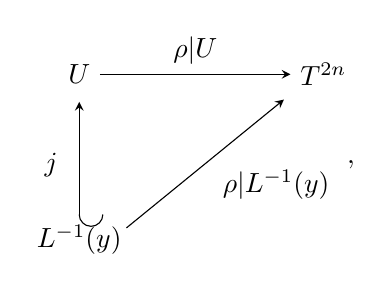
\begin{tikzpicture}[>=stealth]
  \node (U) at (0,0) {$U$};
  \node (T) at (3.1,0) {$T^{2n}$};
  \node (Lm) at (0,-2.1) {$L^{-1}(y)$};
  \draw[->] (U) -- node[above]{$\rho|U$} (T);%
  \draw (0.3,-1.78) arc (0:-180:0.15);%
  \draw[->] (0,-1.78) -- (0,-0.35);%
  \node[left] at (-0.15,-1.15) {$j$};
  \draw[->] (0.6,-1.95) -- (2.6,-0.32);%
  \node[right] at (1.7,-1.4) {$\rho|L^{-1}(y)$};
  \node at (3.45,-1.15) {$,$};%
\end{tikzpicture}
\end{center}
的交换性得出 $(\rho|U)^{*}$ 也是单射，此处 $j$ 表示\trInclusionMapping。这对%
\trCompact{}集 $X_{T}$ 的每个开\trNeighborhood{} $U$ 都成立。于是，利用%
\trAlexander-\trSpanier{}上同调的\trContinuity
\begin{equation}\label{eq:torus-direct-limit}
\check{H}^{*}(X_{T})\ =\ \operatorname{dir.\,lim}\ \check{H}^{*}(U)\,,
\end{equation}
其中这个直极限取遍 $X_{T}$ 的一切\trNeighborhood{} $U$（见附录 8\footnote{原书引作「Appendix 7」，编号有误——直极限构造属附录 8——此处径改实标。——译者注}），我们便%
得到 $(\rho|X_{T})^{*}$ 确实如命题所断言是单射。剩下要证明 \eqref{eq:torus-rho-injective}%
的单射性。

由于 $y$ 是 $L$ 的正则值，映射 $\rho:=\rho|L^{-1}(y):L^{-1}(y)\to T^{2n}$ 是%
两个 $2n$ 维\trCompact\trManifold{}之间的映射。我们将证明
\begin{equation}\label{eq:torus-degree-rho}
\deg_{2}(\rho)\ =\ 1\,.
\end{equation}
取 $\rho$ 的一个正则值 $m\in T^{2n}$。我们断言 $(y,m)$ 是 $(L,\rho)$ 的正则值。%
的确，若 $(L,\rho)(u)=(y,m)$，则 $\widehat{L}'(u):\widehat{\mathcal{B}}\to%
\widehat{\mathcal{E}}$ 是满射，因为按假设 $y$ 是 $L$ 的正则值。注意%
$\ker L'(u)=T\bigl(L^{-1}(y)\bigr)$。由于按假设 $m$ 对 $\rho$ 是正则的，%
\trLinear{}映射 $\rho'(u):T\bigl(L^{-1}(y)\bigr)\to T(T^{2n})$ 是双射。于是，%
相应切空间之间的\trLinear{}映射 $(L'(u),\rho'(u)):\widehat{\mathcal{B}}\to%
\widehat{\mathcal{E}}\times\R^{2n}$ 也是双射，故 $(y,m)$ 如所断言是正则的。%
因此由\cref{prop:smale-degree-one}我们有
\[
\begin{aligned}
1\ \ &=\ \#\ \bigl\{(L,\rho)^{-1}(y,m)\ \bigr\}\quad\text{mod }2\\
&=\ \#\ \bigl\{(\rho|L^{-1}(y))^{-1}(m)\ \bigr\}\quad\text{mod }2\,.
\end{aligned}
\]
由于 $m$ 是正则的，便得出如 \eqref{eq:torus-degree-rho} 所断言的%
$\deg_{2}(\rho)=1$。

把\trCompact{}的 $2n$ 维\trManifold{} $L^{-1}(y)$ 缩记为 $M$，我们以 $o_{M}$%
与 $o_{T}$ 分别表示 $M$ 与 $T^{2n}$ 的 $\Z_{2}$ \trFundamentalClass。鉴于%
\eqref{eq:torus-degree-rho}，由 $\Z_{2}$ 度的同调定义（见附录 7）我们得出
\begin{equation}\label{eq:torus-fundamental-class}
\rho_{*}(o_{M})\ =\ o_{T}\,.
\end{equation}
我们指出：在\trSmooth\trCompact\trManifold{}上，通常的上同调理论（如奇异%
上同调、\trAlexander-\trSpanier{}上同调、\trCech{}上同调）自然\trIsomorphic，%
参见 F.~\trWarner{} [219]。因此，我们可以用奇异上同调代替\trAlexander-\trSpanier{}%
上同调。于是按\trPoincare{}对偶我们有同构
\[
H^{i}(M)\ \xrightarrow{\ \cap o_{M}\ }\ H_{2n-i}(M)\qquad:\qquad%
\alpha\ \mapsto\ \alpha\cap o_{M}\,.
\]
\[
H^{i}(T^{2n})\ \xrightarrow{\ \cap o_{T}\ }\ H_{2n-i}(T^{2n})\qquad:\qquad%
\beta\ \mapsto\ \beta\cap o_{T}\,.
\]
取 $\alpha\in H^{i}(T^{2n})$，我们必须证明 $\rho^{*}(\alpha)=0$ 蕴含 $\alpha=0$。%
为此目的我们考虑映射的复合
\[
H^{i}(T^{2n})\ \xrightarrow{\ \rho^{*}\ }\ H^{i}(M)\ \xrightarrow{\ \cap o_{M}\ }\ %
H_{2n-i}(M)\ \xrightarrow{\ \rho_{*}\ }\ H_{2n-i}(T^{2n})\ %
\xrightarrow{\ (\cap o_{T})^{-1}\ }\ H^{i}(T^{2n})\,.
\]
利用\trCapProduct{}的自然性（见 A.~\trDold{} [62]）并利用 \eqref{eq:torus-fundamental-class}，%
我们算得
\[
\begin{aligned}
&(\cap o_{T})^{-1}\ \rho_{*}\bigl\{(\rho^{*}\alpha)\cap o_{M}\bigr\}\ =\\
&(\cap o_{T})^{-1}\ \bigl\{\alpha\cap\rho_{*}(o_{M})\bigr\}\ =\\
&(\cap o_{T})^{-1}\ \bigl\{\alpha\cap o_{T}\bigr\}\ =\ \alpha\,.
\end{aligned}
\]
从而若 $\rho^{*}\alpha=0$ 则 $\alpha=0$，这证明了 $\rho^{*}$ 是单射。%
\cref{prop:rho-injective-xt}的证明完毕。
\end{proof}

我们现在回到\trBounded{}解之集 $X_{\infty}$，并证明它是一个\trCompact{}集，%
当 $T$ 大时它可以被 $X_{T}$「\trApproximation」。

\begin{proposition}\label{prop:xinf-compact-space}
空间 $X_{\infty}$ 是一个\trCompact{}（度量）空间。
\end{proposition}

\begin{proof}
若 $u\in X_{\infty}$，则当 $s\to\pm\infty$ 时 $u(s)\to\operatorname{Cr}(\varphi)$。%
由于 $\sup\{\,|b(u)|,\ u\in\widehat{\Omega}\,\}<\infty$，由 $\varphi(u(s))$ 的%
\trMonotonicity{}可知存在常数 $C>0$ 满足
\begin{equation}\label{eq:torus-phi-bounded}
-C\ \leq\ \varphi\bigl(u(s)\bigr)\ \leq\ C
\end{equation}
对一切 $u\in X_{\infty}$ 与一切 $s\in\R$。从而集合 $X_{\infty}$ 是闭的。由%
\trVariationOfConstantsFormula{} \eqref{eq:torus-variation-constants}，对每个%
$T>0$ 我们得出
\begin{equation}\label{eq:torus-u0-plus}
u(0)^{+}\ =\ e^{-T}u(-T)^{+}\ +\ P^{+}\int_{-T}^{0}e^{s}\,b'\bigl(u(s)\bigr)\,ds\,.
\end{equation}
由于当 $|s|\to\infty$ 时 $u(s)\to\operatorname{Cr}(\varphi)$，集合 $u(\R)$ 有界，%
于是当 $T\to\infty$ 时我们得出
\begin{equation}\label{eq:torus-u0-plus-limit}
u(0)^{+}\ =\ P^{+}j^{*}\int_{-\infty}^{0}e^{s}\,\nabla b\bigl(u(s)\bigr)\,ds\,.
\end{equation}
对 $u(0)^{-}$ 类似的公式也成立，因此我们可以找到一个\trCompact{}集%
$K\subset T^{2n}\times E$ 使得 $u(0)\in K$ 对一切 $u\in X_{\infty}$。从而集合%
$\{\,u(0)\,|\,u\in X_{\infty}\,\}$ 是\trCompact{}的。由于在 $C^{\infty}$-\trTopology{}%
中解 $u$ 连续依赖于其初值，我们得出 $X_{\infty}$ 也是\trCompact{}的，证明完毕。
\end{proof}

若 $u\in X_{T}$，则按定义 $u$ 是\trGradient{}方程在 $|s|\leq T$ 上的解；于是%
鉴于 $\nabla\varphi$ 的整体\trLipschitz{}连续性，它有唯一的\trContinuation，%
成为对一切时间 $s\in\R$ 有定义的解 $u(s)$。这就定义了一个\trInclusionMapping{}%
$j:X_{T}\to C^{\infty}(\R,T^{2n}\times E)$\footnote{原书印作%
$C^{\infty}(\R,T^{2n}\times\R)$，依下句（$X_{T}$ 视为 $C^{\infty}(\R,T^{2n}\times E)$%
之子集）应为 $E$ 之误，此处径改。——译者注}，下文借此我们可以把 $X_{T}$ 视为%
$C^{\infty}(\R,T^{2n}\times E)$ 的子集。

\begin{proposition}\label{prop:xt-in-neighborhood}
若 $U$ 是 $X_{\infty}$ 的一个开\trNeighborhood，则
\[
X_{T}\ \subset\ U
\]
对充分大的 $T$ 成立。
\end{proposition}

\begin{proof}
由于 $b$ 把 $\widehat{\Omega}$ 映入一个有界集，存在常数 $C>0$ 使得
\begin{equation}\label{eq:torus-phi-restriction}
\varphi\big|E^{-}\ \leq\ C\qquad\text{而}\qquad\varphi\big|E^{+}\ \geq\ -C\,.
\end{equation}
从而，若 $u\in X_{T}$，则
\begin{equation}\label{eq:torus-phi-xt}
-C\ \leq\ \varphi\bigl(u(s)\bigr)\ \leq\ C\,,
\end{equation}
对一切 $u\in X_{T}$、一切 $|s|\leq T$ 与一切 $T>0$。这是因为 $u(s)$ 是负%
\trGradient{}方程 \eqref{eq:torus-gradient-flow} 的解，从而 $\varphi(u(s))$ 是%
一个\trMonotone{}递减函数。我们还得出：存在常数 $M>0$ 使得
\begin{equation}\label{eq:torus-norm-bound}
\|u(-T)\|\ +\ \|u(T)\|\ \leq\ M
\end{equation}
对 $u\in X_{T}$ 与一切 $T>0$。为完成命题的证明，我们反证：假设存在序列%
$T_{n}\to\infty$ 与序列 $u_{n}\in X_{T_{n}}$ 满足 $u_{n}\notin U$。我们将证明%
$u_{n}(0)$ 的一个子序列\trConverge{}到一个点 $x\in T^{2n}\times E$，并且有一条%
\trBounded\trOrbit{} $u\in X_{\infty}$ 经过它。的确，由 \eqref{eq:torus-norm-bound}%
结合 \eqref{eq:torus-u0-plus}，如在\cref{prop:xinf-compact-space}的证明中那样，%
对某个\trCompact{}集 $K^{+}$，当 $n\to\infty$ 时有 $\operatorname{dist}%
\bigl(u_{n}(0)^{+},K^{+}\bigr)\to0$。对 $u_{n}(0)^{-}$ 同理；于是取子序列%
$u_{n}(0)\to x\in T^{2n}\times E$。由 \eqref{eq:torus-phi-xt}，对每个 $n$ 我们有%
$-C\leq\varphi(u_{n}(s))\leq C$（$|s|\leq T_{n}$），其中常数 $C$ 与 $n$ 无关。%
对经过 $x=u(0)$ 的解 $u(s)$ 我们得出 $-C\leq\varphi(u(s))\leq C$ 对一切%
$s\in\R$，因而 $u\in X_{\infty}$。于是，鉴于 $C^{\infty}(\R,T^{2n}\times E)$ 的%
\trTopology{}以及解对初值的连续依赖性，$u_{n}\in U$ 对大的 $n$。这个矛盾%
证明了命题。
\end{proof}

\emph{\cref*{thm:torus-cohomology-injective}的证明（完）。}\quad 为证明%
$(\rho|X_{\infty})^{*}$ 的单射性，取 $X_{\infty}$ 的任一开\trNeighborhood{} $U$。%
由\cref{prop:xt-in-neighborhood}我们有 $X_{T}\subset U$。由%
\cref{prop:rho-injective-xt}，映射 $(\rho|X_{T})^{*}:\check{H}^{*}(T^{2n})\to%
\check{H}^{*}(X_{T})$ 是单射，从而 $(\rho|U)^{*}:\check{H}^{*}(T^{2n})\to%
\check{H}^{*}(U)$\footnote{原书印作 $H^{*}(U)$，脱 Čech 符号；按%
\eqref{eq:torus-direct-limit} 之直极限取遍诸 $\check{H}^{*}(U)$，此处应为%
$\check{H}^{*}(U)$，径改。——译者注}%
是单射。这对\trCompact{}集 $X_{\infty}$ 的每个开\trNeighborhood{}都成立，于是%
我们再次由\trAlexander-\trSpanier{}上同调的\trContinuity{}得出：%
$(\rho|X_{\infty})^{*}:\check{H}^{*}(T^{2n})\to\check{H}^{*}(X_{\infty})$ 是单射。%
\cref{thm:torus-cohomology-injective}的证明完毕。
\end{proof}

\textbf{\trhRemark。}\quad 应当指出，\trTorus{}情形容许更初等的证明。%
\trConley{}与\trZehnder{}在 [55] 中的原始证明同样基于\trLoopSpace{}上的%
\trHamiltonian{}变分函数。然而，利用覆盖空间的线性结构、十分特殊的%
\trSymplecticStructure{} $\omega_{0}$ 以及\trTorus{}的\trCompactness，在无穷维%
\trLoopSpace{}上寻找\trCriticalPoint{}的问题被化归为在\trTorus{}的一个有限维%
\trBundle{} $T^{2n}\times\R^{N}$ 上寻找相关\trFunctional{}的\trCriticalPoint{}的%
等价问题。这里维数 $N$ 很大，并且当然依赖于所考虑的\trHamiltonianFunction{}%
$H$。所用的约化是所谓的\trLyapunov-\trSchmidt{}\trReduction，它是泛函分析中一种众所周知%
的技术。问题随之而来：是否存在内在的有限维方法？的确，M.~\trChaperon{}在%
[43]（1984）中找到了另一个变分泛函，它借一个由有限个\trGeneratingFunction{}%
构成的序列直接定义在\trTorus{}的一个有限维向量丛上。他还把他的「破裂\trGeodesic{}%
方法」应用到 $T^{*}(T^{n})$ 中\trLagrange{}子流形的几何整体相交问题。他证明：%
$T^{*}(T^{n})$ 的\trHamiltonianMap{} $\varphi$ 永远不能把与 $T^{n}$%
\trDiffeomorphic{}\trZeroSection{} $0^{*}_{T^{n}}$ 从其自身分离出来。更精确地，他证明了
\[
\#\ \{\ T^{n}\cap\varphi(T^{n})\ \}\ \geq\ \text{\trCupLength}\,(T^{n})\ +\ 1\,,
\]
（若相交是横截的，则 $\geq SB(T^{n})$）。这是 V.I.~\trArnold{}在 [9] 中提出的%
一个长期悬而未决的问题。关于这一变分方法的修改与进一步应用，参见%
[41]--[44]。这里我们还要提到 A.B.~\trGivental{} [105]、M.~\trBrunella{} [36] 与%
Yu.~V.~\trChekanov{} [47]。J.C.~\trSikorav{} [197]（1987）的相关有限维方法基于%
\trLagrange{}流形的生成\trPhaseFunction{}这一概念。这个概念较早出现在\trFourierIntegralOperator{}的%
理论中，参见 L.~\trHormander{} [124]。这种优美的方法结果证明对特殊%
\trSymplecticManifold{} $(T^{*}M,d\lambda)$ 特别有用，正如\trHofer{}拉格朗日%
相交定理在 $T^{*}M$ 中对一般\trCompact\trManifold{} $M$ 的新证明所展示的那样——%
它推广了上面的\trTorus{}情形，参见 [197, 136]。该结果早先由 H.~\trHofer{}%
[114]（1985）发现。它陈述：对 $(T^{*}M,d\lambda)$ 的每个\trHamiltonianMap{}%
$\varphi$，
\[
\#\ \{\ M\cap\varphi(M)\ \}\ \geq\ \text{\trCupLength}\,(M)\ +\ 1\,,
\]
此处我们已把 $M$ 等同于\trZeroSection $0^{*}_{M}$。

在有限维变分论证的这一背景中，我们还应提到：C.~\trViterbo{}在其工作「辛拓扑%
作为生成函数的几何」[218]（1992）中，把\trLagrange{}子流形的辛容量定义为相关%
\trPhaseFunction{}的\trCriticalValue。这样，他便利用那些作为具\trCompactSupport{}的%
\trHamiltonian{}映射之图像的\trLagrange{}子流形，定义了 $(\R^{2n},\omega_{0})$ 的%
开子集的容量。Ya.~\trEliashberg{}在其 1992 年的讲学中勾画了如何把%
\trViterbo{}的方法扩展成 6.6 节所描述的\trFloer-\trHofer\trSymplectic\trHomology{}%
理论的一个替代构造——针对 $(\R^{2n},\omega_{0})$ 的开子集这一特殊情形。其%
构造的细节最近由 L.~\trTraynor{}在预印本「借生成函数的辛同调」[212] 中完成。

似乎迄今引入的这些有限维变分方法并不适合一般的\trSymplecticManifold。%
因此，我们上面把\trTorus{}情形的证明建立在\trLoopSpace{}中的\trAction{}原理%
之上。我们的证明表明：变分原理的关键信息包含在人为\trGradient{}流的%
\trBounded{}解之集中。这个集合由\trRestPoint{}连同\trConnectingOrbit{}组成。%
这一观察对于\trFloer{}处理下述\trFunctional{}的\trMorseTheory{}将颇为要紧：%
这些\trFunctional{}的\trGradient{}甚至不生成\trFlow。
